\documentclass[11pt,a4paper]{report}
\usepackage{listings}
\usepackage{subfig}
\usepackage{booktabs}
\usepackage{amsmath}
\usepackage{setspace}
\usepackage{graphicx}
\usepackage{warwickthesis}
\usepackage{natbib}
\usepackage[toc,page]{appendix}

% Configure listings
\lstset{
frame=tblr,
basicstyle=\small,
}

%\usepackage[font=footnotesize,margin=15pt,textfont=sl]{caption}


% These come from warwickthesis.sty
\phdthesis
\thesisdraft
\leftchapter
\onehalfspacing


\begin{document}

%\maketitle

\chapter{NGTS error budget}

The NGTS instrument is a new robotic telescope under construction at
Paranal in Chile. It is a system of 12 automated telescopes which survey
the sky searching for extrasolar transiting planets around $9$-$15$th
magnitude stars. The observations are made using a red filter ($\sim
500$-$850$nm) so are affected by the higher level of sky background.
Considerations about the technology and observational strategy, along
with the long prototyping stage have lead to the project pushing the
boundaries of precision for an instrument of its type and so a thorough
investigation of the noise sources is required.

Transiting extrasolar planets are easiest to find around bright 
stars due to the high signal to noise ratio from the source. The noise
factor for these objects is dependant on a few usually observational
effects; such as the level of the sky background, or read noise; and the
noise from the object itself. The noise to signal ratio gives the amount
of noise from a noise source as a fraction of the detected flux from
that source and is a natural way of considering noise sources and which
is dominant. 

The need to include bright stars coupled with the need to reduce noise
means an optimisation of the instrumental settings (gain, readout speed)
and observational conditions (exposure time) to provide the best planet
searching opportunities.

\section{Noise sources}

The noise in a CCD image comes from four main sources (assuming all
units are electrons):

\begin{itemize}
    \item Poisson noise from the source ($\sigma_{\ast}$). This is 
        just due to the counting statistics of the number of
        photons from the source:

        \[
            \sigma_{\ast} = \sqrt{N_{\ast}}
            \]

    \item Poisson noise from the sky ($\sigma_s$). Again counting 
        statistics but from the sky

        \[
            \sigma_{s} = \sqrt{N_{s}}
            \]

        The number of counts is required for the source aperture, but is
        usually calculated from the sky annulus. Therefore to convert
        from one to another:

        \[
            N_s = \frac{n_{sci}}{n_{sky}} N_{\mathrm{per pix}}
            \]

    \item Read noise from the CCD electronics ($\sigma_R$). This is 
        usually given by the specifications sheet for a camera
        but can also be measured, and is given in electrons per pixel.
        This value does not change with exposure time and is just added
        with every exposure. 

    \item Scintillation noise from the atmosphere
        ($\sigma_{\mathrm{scin}}$). The error on this is given by
        \citet{southworth09}:


        \[
            \sigma_{\mathrm{scin}} = 0.004
            D^{-2/3}X^{7/4}\exp{-h/H}\left(2t_e\right)^{-1/2}
            \label{eq:scintillation}
            \]

        where $D$ is the aperture size in m, $X$ is the airmass, $h$ is
        the height above sea level of the observations, $H$ is the scale
        height ($= 8000$m), and $t_e$ is the exposure time.
\end{itemize}

These noise sources can be reduced by two methods:

\begin{itemize}
    \item Taking longer exposures. The scintillation noise directly
        decreases by $t_e^{-1/2}$. The other noise sources increase less
        quickly when compared to the signal and so the noise to signal
        ratio reduces.
    \item Combining images. This is in effect the same as the previous
        method but a shorter exposure time allows for a brighter
        saturation limit. The downside of this is that the readout time
        at short exposures becomes a large fraction of the total frame
        capture time and is therefore equivalent to not observing for a
        fraction of time.
\end{itemize}

Estimating which method is preferable is the subject of the next
section.



\section{Flux fraction}
\label{sec:ffraction}

When a psf is centred on a pixel, the largest amount of flux enters that
pixel. This is a very pessimistic aproach since this will cause more
stars to saturate than is realistic due to the nature of the placement
of the stars. To find the most likely value of this fraction, a Gaussian
psf was simulated at a random offset within the pixel value.
$1\times10^6$ offsets were chosen within a range $-0.5 < x < 0.5$ and
$-0.5 < y < 0.5$ and the integral recalculated. The fractional values
were binned up and the bin values were divided by the total number of
iterations giving the probability density. The most likely value was
calculated from this and used in the analysis in the main text.
Figure~\ref{fig:fractiondistribution} shows the resulting distribution.

\begin{figure}[h]
    \begin{center}
        \includegraphics[angle=270,width=0.9\columnwidth]{images/fractiondistribution}
    \end{center}
    \caption{Distribution of the flux fraction in the central pixel as
    an aperture is randomly offset. The most likely value is plotted.}
    \label{fig:fractiondistribution}
\end{figure}

\section{Sky background}

The sky background level is very dependant on the amount of light due to
the Moon is visible in the image. This is loosely related to the phase
of the Moon, but not completely since the chosen field might not be
within the Moon avoidance area.

The median image level for each image of the NGTS prototype data set was
used to estimate the sky background level, and the value divided by the
exposure time to give the ADU per second. This was scaled by the gain
$1.2 e^{-1} \mathrm{ADU}$ to give electrons per second per pixel for
each image. The JD was also recorded and used to calculate the phase of
the Moon for each image. 

The Moon avoidance angle describes the angular distance from the Moon in
which the Moon light is present. The Moon phase therefore is not the
only indicator: the Moon could be full but the field being observed may
be outside the Moon avoidance angle. Therefore there is some scatter, as
can be seen in fig.~\ref{fig:skyvsmoon}.

\begin{figure}[h]
    \begin{center}
        \includegraphics[angle=270,width=0.9\columnwidth]{images/skyvsmoon}
    \end{center}
    \caption{Sky background level per pixel per second for the NGTS
    prototype data plotted against Moon phase. A linear fit is made only to
indicate the trend.}
    \label{fig:skyvsmoon}
\end{figure}










\section{Noise on transit timescales}

The noise sources were combined using the methods outlined in section
\ref{sec:method} to provide the level of noise as a function of sky
exposure time (exposure time not devoted to reading out the ccd). The
source flux is input as a source magnitude and converted to photons. The
zero point of NGTS data is calibrated to catalogue stars (in the I band,
the closest matching band to the instrument). The flux received in one
second is given by:

\[
    m = m_0 - 2.5 \log_{10}{f}
    \]

\[
    m_0 - m = 2.5 \log_{10}{f}
\]

\[
    f = 10^{(m_0 - m) / 2.5}
    \]

To include the extinction from the atmosphere, a constant correction
term is added to the magnitude value so that 

\[
    m = m_0 - 2.5 \log_{10}{f} - k X
    \]

where $k$ is the extinction coefficient ($\sim 0.06$ for NGTS), and $X$
the airmass. This assumes a measured flux $f$ and corrects for the atmosphere to give
the magnitude as would be observed from space. For this analysis the
magnitude specified at the program start is the magnitude that would be
observed from space and the flux recieved through the atmosphere at
airmass $X$ is what's needed. Therefore the last term is inverted, and
the final flux value is given by 

\[
    f = 10^{(m_0 + k X - m) / 2.5}
    \]


\subsection{Method}
\label{sec:method}

Exposures were simulated for a particular sky exposure time ($t_e$), 
but the
readout time was included to calculate the number of exposures that
would be taken in a total of one hour, the typical timescale of a
planetary transit, with the sky exposure time ranging from $5$ to $3600$
seconds. . The total readout time is a combination of the number
of pixels and the vertical and horizontal readout times. The vertical
time is set by the manufacturer but the horizontal readout \emph{speed}
can be altered by the user. The NGTS cameras have three settings: $1$,
$3$ and $5$ MHz, with $3$ MHz chosen for this study. The vertical
readout time is given as $38 \mu\mathrm{s}$. The frame read time is
therefore

\[
    t_R = \mathrm{naxis2} \left[t_v + \frac{\mathrm{naxis1}}{\nu_H}\right]
    \]

where naxis1, naxis2 are the number of pixels in each dimension of the
CCD, $t_v$ is the vertical readout time and $\nu_H$ is the horizontal
readout speed. Table \ref{tab:ccdparams} gives the specifications for
the NGTS cameras and the readout time is calculated at $1.49$ seconds.

\begin{table}
    \centering
    \begin{tabular}{ccr}
        \toprule
        Parameter & Value & Unit \\
        \midrule
        $\nu_H$ & $3$ & MHz \\
        $t_v$ & $38$ &  $\mu s$ \\
        naxis1 & 2048 & pixels \\
        naxis2 & 2048 & pixels \\
        \midrule
        $t_R$ & 1.49 & s \\
        \bottomrule
    \end{tabular}
    \caption{CCD characteristics for the NGTS cameras. Derived
    parameters are below the horizontal line.}
    \label{tab:ccdparams}
\end{table}

The total exposure time is given by 

\[
    t_T = t_e + t_R
    \]


The number of exposures that can be taken in one hour is therefore 

\[
    n_{e} = \frac{3600}{t_T} = \frac{3600}{t_e + t_R}
    \]

Each noise source per image is then combined using $n_e$ exposures into
a combined hour long exposure. The method of combining the  noise sources 
will now be explained in turn.

\subsubsection{Poisson sources (source and sky noise)}

For an exposure time of $t_e$ the number of source counts is given by

\[
    N_{\ast} = N_{\ast,\mathrm{per sec}} t_e
    \]

The error from the source noise is therefore
\[
    \sigma_{\ast} = \sqrt{N_{\ast}} = \sqrt{N_{\ast,\mathrm{per sec}}}
    \times \sqrt{t_e}
    \]

When combining images, the error per image is the same so summing
variances:

\begin{align*}
    \sigma_{\ast,T}^2 &= \sum_i^{n_{e}} \sigma_{\ast,i}^2 \\
        & = n_{e} \sigma_{\ast,i}^2
\end{align*}

\[
    \sigma_{\ast, T} = \sqrt{n_{e}} \sigma_{\ast}
    \]

The analysis of the sky noise follows a similar procedure, but requires
calculating the sky counts in an aperture around the target star, given
by

\[
    n_{s} = \pi r^2
    \]

where $n_s$ is the number of pixels and $r$ is the radius of the
aperture. General consensus is that the aperture size should be a
multiple of the FWHM of the optical psf of the instrument. The NGTS psf
has a FWHM of around 1.5 pixels and an aperture radius of two pixels was
used, giving a total number of aperture pixels as $n_s = \pi 1.5^2 =
12.56$ pixels. The sky counts per pixel per second can be multiplied by
this factor to get the sky counts per second. The analysis from this
point on is identical to that of the source error outlined above.

\subsubsection{Read noise}

The read noise is quoted as electrons per pixel. For an aperture with
area $A$ the errors are added in quadrature for each pixel to give for a
single exposure:

\[
    \sigma_{R,\mathrm{pi}}^2 = A N_{R,pp}^2
    \]

\[
    \sigma_{R,\mathrm{pi}} = \sqrt{A} N_{R,pp}
\]

where $pp$ indicates per pixel and $pi$ indicates per image. These 
are then combined for each exposure to give a total read noise 
level of 

\[
    \sigma_{R,T} = \sqrt{A n_e} N_{R,pp}
    \]


\subsubsection{Scintillation noise}

The error in magnitudes for the scintillation is given by
eq.~\ref{eq:scintillation} and is already the fractional error due to
scintillation. When coadding frames however the number of photons due to
scintillation must be used so the fractional error given by
eq.~\ref{eq:scintillation} is multiplied by the source counts for each
frmae and then coadded.

\[
    \sigma_{\mathrm{scin}} = \sigma_{\mathrm{scin},\mathrm{frac}} N_{\ast}
    \]

\[
    \sigma_{\mathrm{scin},T} = \sqrt{n_e} N_{\mathrm{scin}} 
\]

Table~\ref{tab:scintillationparams} gives the required constants for
eq.~\ref{eq:scintillation}.


\begin{table}
    \centering
    \begin{tabular}{ccr}
        \toprule
        Parameter & Value & Unit \\
        \midrule
        D & 0.2 & m \\
        h & 2400 & m \\
        X & 1 or 2 & - \\
        \bottomrule
    \end{tabular}
    \caption{Parameters for the scintillation calculation at Paranal.}
    \label{tab:scintillationparams}
\end{table}


\subsubsection{Total noise}

After the sources of noise are calculated for the combined hour long 
exposures (either through direct sky exposure time or coadding 
exposures), the combined error from all of the sources can be
calculated:

\[
    \sigma_T = \sqrt{\sigma_{\ast,T}^2 + \sigma_{s,T}^2 + \sigma_{R,T}^2 +
    \sigma_{\mathrm{scin},T}^2}
    \]





\subsection{Saturation}

A pixel will saturate if the number of counts is greater than its 
full well depth. For NGTS this value is $150000$ electrons. To 
estimate the saturation point, the number of photons that fall on 
a single pixel for a given brightness must be calculated. 

Assuming the worst case where the psf of an object is centered on 
a pixel, the fraction of light that falls in this pixel is given 
by the ratio of the integral of the psf inside that central pixel to
the integral of the full psf. Assuming a Gaussian psf, this fraction is

\[
    F = \frac{\int_{-0.5}^{0.5}\int_{-0.5}^{0.5} G(x,y) dx dy}
    {\int_{-\infty}^{\infty}\int_{-\infty}^{\infty} G(x,y) dx dy}
    \]

where $G$ is a 2D Gaussian function centered on $0$ with a standard
deviation of $\sigma$:  

%\[
%    G = e^{-0.5 ((x/\sigma) + (y/\sigma)}
%    \]

\[
G(x,y) = \exp \left[
		-\frac{1}{2\sigma^{2}} \left(
			x^{2} + y^{2}
		\right)
	\right]
\]

The FWHM of a Gaussian function is $\sim 2.35 \sigma$ which is used to
convert from the psf width. This ratio was calculated through numerical
integration with the trapezium method on a computer and equates to $\sim
0.32$ for a FWHM of 1.5 pixels. This value is the worst case, so for an
explanation of a more realistic assessment, see appendix \ref{sec:ffraction}.


To calculate the saturation point, the total number of photons comes
from three sources: the source, the sky and the bias level. The bias
level is a deliberate offset applied to the image to prevent negative
numbers being recorded which due to the digitisation process would cause
undefined behaviour. The typical level is around 900 electrons and is
set by the readout software. Once the total number of electrons recorded
for an aperture multiplied by the fraction of light in the central pixel
reaches the full well depth then the central pixel becomes saturated.
The saturation level is therefore given by

\[
    L_{\mathrm{sat}} = F  (N_{\ast} + N_{s} + N_{b})
    \]



\subsection{Results}

At low sky exposure times the readout time becomes a significant fraction of the total exposure time so the number of photons collected is lower, which leads to a higher than usual fractional noise level shown in fig.~\ref{fig:brightnoise} at exposures of less than $10$s.

\begin{figure}[h]
    \begin{center}
        \includegraphics[angle=270,width=0.9\textwidth]{images/bright}
    \end{center}
    \caption{Noise contributions for the NGTS instrument. All sources
    are combined up to a total exposure time of one hour. Each source is
the fraction of the total counts recieved from the object, for an object
magnitude of 9. The dashed vertical line marks the exposure time at
which the object saturates. Solid lines indicate an airmass of $1$, and
dashed lines indicate an airmass of $2$.}
    \label{fig:brightnoise}
\end{figure}

Between the airmass $1$ and airmass $2$ data, the biggest difference is
in the scintillation level which increases by $2.36$ times.
Scintillation is the dominant source of noise for bright objects and
this becomes more apparent at high airmasses.
Figure~\ref{fig:faintnoise} shows the dominant noise source for a faint
object is the sky background, though at low exposure times the read
noise increases to above the source noise.


\begin{figure}[h]
    \begin{center}
        \includegraphics[angle=270,width=0.9\textwidth]{images/faint}
    \end{center}
    \caption{Equivalent result as fig.~\ref{fig:brightnoise} for a
$15$th magnitude object.}
    \label{fig:faintnoise}
\end{figure}



\section{Saturation level for a given exposure time}
\label{sec:satlevel}

From the previous analysis the saturation level for a given exposure
time can be calculated and modelled. The simulation was run for multiple
exposure times and the saturation level calculated and plotted in
fig.~\ref{fig:satvsexpos}. The simulation was run for bright time and
dark time (based on estimations of the background at differing Moon
phases) and a separate fit was made to each.

\begin{figure}[h]
    \begin{center}
        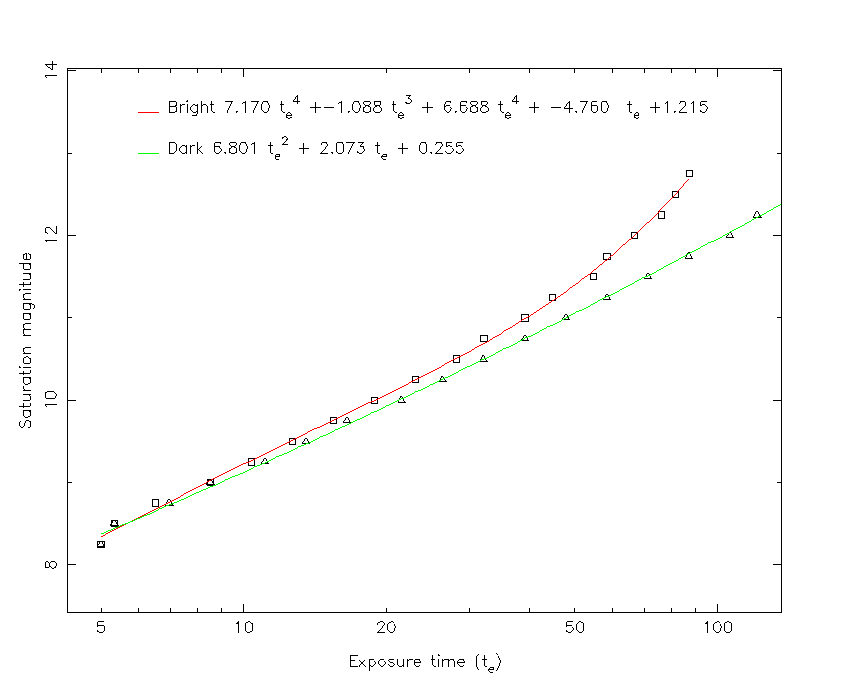
\includegraphics[angle=270,width=0.9\textwidth]{images/satvsexpos}
    \end{center}
    \caption{}
    \label{fig:satvsexpos}
\end{figure}


If a source increases in flux by $100$ times the magnitude by definition
decreases by $5$. This predicts linear behaviour in $\log_{10}{f}$ but
clearly the lines are best modelled by $4$th and $2$nd order
polynomials. This deviation is due to the extra sources of noise
contributing. The least squares fits are displayed on fig.~\ref{fig:satvsexpos}, 
and the coefficients are displayed in table~\ref{tab:coeffs} for the formula:

\[
L_{\mathrm{sat},\mathrm{j}} = \sum_{i=0}^{4} a_{i,j} t_{e}^{i}
\]

where $j$ is bright or dark.

%\[
%    L_{\mathrm{sat},\mathrm{bright}} = 9.503 t_e^4 - 8.423 t_e^3 +
%    13.737 t_e^2 - 7.502 t_e + 1.54
%    \]
%
%\[
%    L_{\mathrm{sat},\mathrm{dark}} = 6.758 t_e^2 + 1.691 t_e + 0.352
%\]

\begin{table}[htbp]
   \centering
   \begin{tabular}{@{} ccc @{}} % Column formatting, @{} suppresses leading/trailing space
      \toprule
      Coefficient & Bright value & Dark value \\
            \midrule
	$a_{0}$ & $1.54$ & $0.352$ \\
      $a_{1}$ & $-7.502$ & $1.691$ \\
      $a_{2}$ & $13.737$ & $6.758$ \\
      $a_{3}$ & $-8.423$ & $0$ \\      
      $a_{4}$ & $9.503$ & $0$ \\
      \bottomrule
   \end{tabular}
   \caption{Remember, \emph{never} use vertical lines in tables.}
   \label{tab:coeffs}
\end{table}

\section{Saturated stars in a field}

Using the results from section~\ref{sec:satlevel}, the number of stars
for a given field which are saturated can be estimated using catalogue
information. 

\subsection{Method}

The UCAC-3 catalogue was used to retrieve the magnitudes of all stars
in a list of filters (Johnson-Cousins BRIJHK) but R is the closest match 
to the NGTS filter. 

The area cone search for the catalogue was matched to the field of view
for the instrument to ensure the same density of stars were returned. By
matching the areas:

\[
    A_{\mathrm{fov}} = A_{\mathrm{cone}}
    \]
\[
    \pi R^2 = \mathrm{naxis1} \times \mathrm{naxis2}
    \]

\[
    R = \sqrt{\frac{\mathrm{naxis1} \times \mathrm{naxis2}}{\pi}}
    \]

with $R$ the radius of the cone, and all units in arcminutes. The
saturation level is calculated for a range of exposure times from $5$s
to $3600$ seconds, and the number of objects in the field with
magnitudes higher or equal to this level were counted. Again this
analysis was performed for bright and dark time.

\begin{figure}[h]
    \begin{center}
        \includegraphics[angle=270,width=0.9\columnwidth]{images/totalsaturated}
    \end{center}
    \caption{Total number of saturated stars for three NGTS fields}
    \label{fig:totalsaturated}
\end{figure}


\begin{figure}[h]
    \begin{center}
        \includegraphics[angle=270,width=0.9\columnwidth]{images/fractionsaturated}
    \end{center}
    \caption{Fraction of saturated stars for three NGTS fields}
    \label{fig:fractionsaturated}
\end{figure}



\section{Noise for a given magnitude}
\label{sec:noisepermag}

As can be seen from fig.~\ref{fig:brightnoise} and
fig.~\ref{fig:faintnoise}, the noise levels change dramatically when
going from a magnitude $9$ object to a magnitude $15$ object. For
bright objects, the scintillation is the dominant source of noise,
whereas for faint objects the sky background is the domniant source of
noise. The fractional noise level also changes in absolute terms, 
for example with the sky noise error changing from
$\sim 0.025$ mmag  to $\sim 6$ mmag.


\begin{figure}[p]
  \centering
  \subfloat[$5$s exposure, dark time]{\label{fig:5sdark}\includegraphics[angle=270,width=0.4\textwidth]{images/5sdark}}                
  \subfloat[$5$s exposure, bright time]{\label{fig:5sbright}\includegraphics[angle=270,width=0.4\textwidth]{images/5sbright}} \\               
  \subfloat[$10$s exposure, dark time]{\label{fig:10sdark}\includegraphics[angle=270,width=0.4\textwidth]{images/10sdark}}                
  \subfloat[$10$s exposure, bright time]{\label{fig:10sbright}\includegraphics[angle=270,width=0.4\textwidth]{images/10sbright}} \\               
  \subfloat[$30$s exposure, dark time]{\label{fig:30sdark}\includegraphics[angle=270,width=0.4\textwidth]{images/30sdark}}                
  \subfloat[$30$s exposure, bright time]{\label{fig:30sbright}\includegraphics[angle=270,width=0.4\textwidth]{images/30sbright}}
  \caption{Theoretical error curves for the NGTS instrument. Each line represents a different
  error source, with the combined error shown in black. The plots are
  for $5$, $10$ and $30$ seconds of science exposure, both in dark and
  bright time, and include the
  $\sim 1.5$s frame read time. The horizontal
  line shows the target $1$mmag level, and the vertical line where the
  total error value intercepts the $1$mmag line. The value is quoted in
  the title for each figure.}
  \label{fig:rmsmagplots}
\end{figure}

\begin{table}[h]
    \centering
    \begin{tabular}{ccc}
        \toprule
        Exposure time (s) & Sky type & $1$mmag point \\
        \midrule
        5 & dark & $13.210$ \\
        5 & bright & $12.836$ \\
        10 & dark & $13.384$ \\
        10 & bright & $12.946$ \\
        30 & dark & $13.496$ \\
        30 & bright & $13.023$ \\
        \bottomrule
    \end{tabular}
    \caption{Predicted $1$mmag points for the NGTS instrument}
    \label{tab:1mmagpoints}
\end{table}


To investigate this, the noise levels were calculated for a range of
magnitudes covering the NGTS visible range. As a theoretical
investigation the range goes brighter than the saturation limit of NGTS
and fainter than the detection limit, and each error contribution has
been combined up to an hour as in previous investigations to ascertain
the error expected on transit-like timescales.
Figure~\ref{fig:rmsmagplots} shows the results, and the magnitude at
which the precision is $1$mmag  is listed in table~\ref{tab:1mmagpoints}



\section{Storage requirements}

For financial reasons, the number of images taken per year must be
estimated as hard disk storage is expensive in large quantities. The
number of calibration frames (assuming only dark, bias and flat frames
are required) and science frames for a given exposure time are
calculated. 


\subsection{Calibration frames}


\subsection{Science images}

\subsection{Total}


\bibliographystyle{plainnat}
\bibliography{bibliography}
\end{document}
